\begin{frame}
	\myheading{Module 19.2: The concept of a latent variable}
\end{frame}

\begin{frame}
	\begin{columns}
		\column{0.4\textwidth}
		\begin{overlayarea}{\textwidth}{\textheight}
		\begin{figure}
		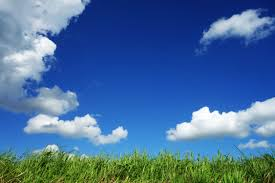
\includegraphics[width=100pt, height=100pt]{images/sunnysky}
		\end{figure}
		\end{overlayarea}
		\column{0.6\textwidth}
		\begin{overlayarea}{\textwidth}{\textheight}
			\begin{itemize}\justifying
				\item<1->We now introduce the concept of a latent variable
				\item<2-> Recall that earlier we mentioned that the neighboring pixels in an image are dependent on each other
				\item<3-> Why is it so? \onslide<4->{(intuitively, because we expect them to have the same color, texture, etc.?)}
				\item<5-> Let us probe this intuition a bit more and try to formalize it
			\end{itemize}
		\end{overlayarea}
	\end{columns}
\end{frame}

\begin{frame}
	\begin{columns}
		\column{0.4\textwidth}
		\begin{overlayarea}{\textwidth}{\textheight}
		\begin{figure}
		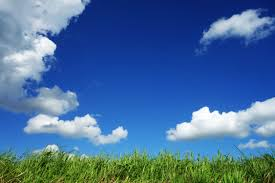
\includegraphics[width=100pt, height=100pt]{images/sunnysky}
		\end{figure}
		\end{overlayarea}
		\column{0.6\textwidth}
		\begin{overlayarea}{\textwidth}{\textheight}
			\begin{itemize}\justifying
			\footnotesize
				\item<1-> Suppose we asked a friend to send us a good wallpaper and he/she thinks a bit about it and sends us this image
				\item<2-> Why are all the pixels in the top portion of the image blue? \onslide<3->{(because our friend decided to show us an image of the sky as opposed to mountains or green fields)}
				\item<4-> But then why blue why not black? \onslide<5->{(because our friend decided to show us an image which depicts daytime as opposed to night time)}
				\item<6-> Okay, But why is it not cloudy (gray)?\onslide<7-> {(because our friend decided to show us an image which depicts a sunny day)}
				\item<8-> These decisions made by our friend (sky, sunny, daytime, etc) are not explicitly known to us (they are hidden from us)
				\item<9-> We only observe the images but what we observe depends on these latent (hidden) decisions
			\end{itemize}
		\end{overlayarea}
	\end{columns}
\end{frame}
\begin{frame}
	\begin{columns}
		\column{0.4\textwidth}
		\begin{overlayarea}{\textwidth}{\textheight}
		\onslide<1->{
		\begin{figure}
		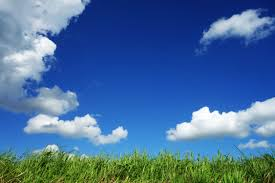
\includegraphics[height=50pt,width=50pt]{images/sunnysky}
		\end{figure}
		\vspace{-0.3in}
		\footnotesize
		\begin{align*}
		\text{Latent Variable} = \text{daytime}
		\end{align*}}
		\vspace{-0.2in}
		\onslide<4->{
		\begin{figure}
		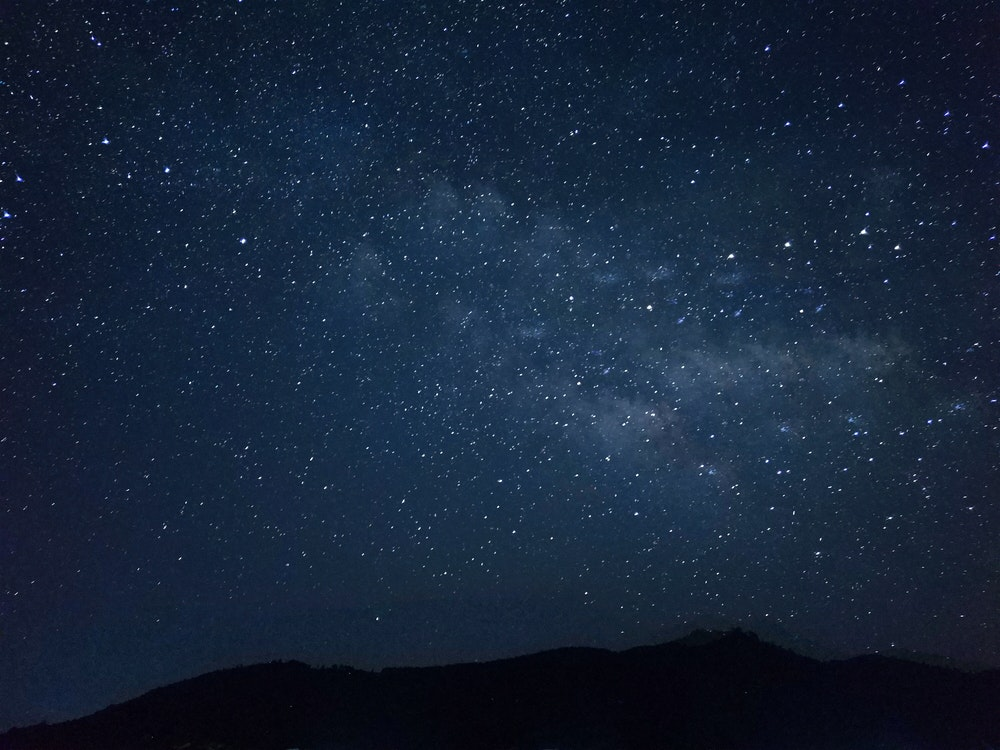
\includegraphics[height=50pt,width=50pt]{images/nightsky}
		\end{figure}
		\vspace{-0.2in}
		\footnotesize
		\begin{align*}
		\text{Latent Variable} = \text{night}
		\end{align*}}
		\vspace{-0.2in}
		\onslide<5->{
		\begin{figure}
		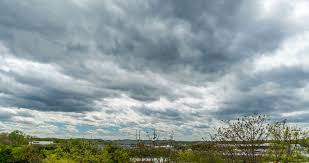
\includegraphics[height=50pt,width=50pt]{images/cloudysky}
		\end{figure}
		\vspace{-0.2in}
		\footnotesize
		\begin{align*}
		\text{Latent Variable} = \text{cloudy}
		\end{align*}}
		\end{overlayarea}
		\column{0.6\textwidth}
		\begin{overlayarea}{\textwidth}{\textheight}
			\begin{itemize}\justifying
				\item<1-> So what exactly are we trying to say here?
				\item<2-> We are saying that there are certain underlying hidden (latent) characteristics which are determining the pixels and their interactions
				\item<3-> We could think of these as additional (latent) random variables in our distribution
				\item<6-> These are latent because we do not observe them unlike the pixels which are observable random variables
				\item<7-> The pixels depend on the choice of these latent variables
			\end{itemize}
		\end{overlayarea}
	\end{columns}
\end{frame}


\begin{frame}[shrink=5]
	\begin{columns}
		\column{0.4\textwidth}
		\begin{overlayarea}{\textwidth}{\textheight}
			\vspace{1cm}

	        \onslide<3->{
	        \tikzset{mystyle/.style={shape=circle,fill=black,scale=0.3}}
			\tikzset{neigh/.style={shape=circle,fill=blue,scale=0.5}}
			\tikzset{cent/.style={shape=circle,fill=red,scale=0.5}}
			\tikzset{hid/.style={shape=circle,fill=green,scale=0.5}}
			\tikzstyle{input_neuron}=[circle,draw=red!50,fill=orange!10,thick,minimum size=3mm]
			\begin{center}
			\begin{tikzpicture}[scale=.7]
            % setup the nodes
          	\node[inner sep=0,opacity=0.3] at (3,3)
			{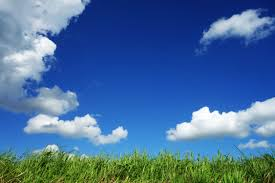
\includegraphics[width=150pt,height=150pt]{images/sunnysky}};

            \onslide<4->{

            \draw[fill=black!30, rounded corners] (0.8, 8.2) rectangle (5.2, 7.8) {};
            \foreach \x in {1,...,5}
            {

            	\draw [->,line width=0.1mm] (\x,8) -- (0,6);
            	\draw [->,line width=0.1mm] (\x,8) -- (1,6);
            	\draw [->,line width=0.1mm] (\x,8) -- (2,6);
            	\draw [->,line width=0.1mm] (\x,8) -- (3,6);
            	\draw [->,line width=0.1mm] (\x,8) -- (4,6);
            	\draw [->,line width=0.1mm] (\x,8) -- (5,6);
            	\draw [->,line width=0.1mm] (\x,8) -- (6,6);
            	\draw [->,line width=0.1mm] (\x,8) -- (0,5);
            	\draw [->,line width=0.1mm] (\x,8) -- (1,5);
            	\draw [->,line width=0.1mm] (\x,8) -- (2,5);
            	\draw [->,line width=0.1mm] (\x,8) -- (3,5);
            	\draw [->,line width=0.1mm] (\x,8) -- (4,5);
            	\draw [->,line width=0.1mm] (\x,8) -- (5,5);
            	\draw [->,line width=0.1mm] (\x,8) -- (6,5);
                \foreach \x in {1,...,5}
            	\foreach \y in {8}
            {
            	\node[hid] (1) at (\x,\y){};
            }}
            }
            \foreach \x in {0,...,6}
            \foreach \y in {0,...,6}
            {
                \node[mystyle] (\x-\y) at (\x,\y){};

            }
            \onslide<3>{
			\foreach \x in {2,3,4}
			\foreach \y in {0,1,2}
			\foreach \a in {2,3,4}
			\foreach \b in {0,1,2}
			{
				\draw [line width=0.2mm,blue, -] (\x,\y) -- (\a,\b);
			}
			\foreach \x in {2,3,4}
			\foreach \y in {4,5,6}
			\foreach \a in {2,3,4}
			\foreach \b in {4,5,6}
			{
				\draw [line width=0.2mm,red, -] (\x,\y) -- (\a,\b);
			}
			\foreach \x in {4,5,6}
			\foreach \y in {2,3,4}
			\foreach \a in {4,5,6}
			\foreach \b in {2,3,4}
			{
				\draw [line width=0.2mm,green, -] (\x,\y) -- (\a,\b);
			}
			}
	        \end{tikzpicture}
	        \end{center}
	        }
		\end{overlayarea}
		\column{0.6\textwidth}
		\begin{overlayarea}{\textwidth}{\textheight}
			\begin{itemize}\justifying
				\item<1-> More formally we now have visible (observed) variables or pixels $(V = \{V_1, V_2, V_3, \dots, V_{1024}\})$ and hidden variables $(H = \{H_1, H_2, ..., H_n\})$
				\item<2-> Can you now think of a Markov network to represent the joint distribution $P(V, H)$?
				\item<3->  Our original Markov Network suggested that the pixels were dependent on neighboring pixels (forming a clique)
				\item<4-> But now we could have a better Markov Network involving these latent variables
				\item<5-> This Markov Network suggests that the pixels (observed variables) are dependent on the latent variables (which is exactly the intuition that we were trying to build in the previous slides)
				\item<6-> The interactions between the pixels are captured through the latent variables
			\end{itemize}
		\end{overlayarea}
	\end{columns}
\end{frame}



\begin{frame}
\begin{block}{}
\begin{itemize}\justifying
\item<1-> Before we move on to more formal definitions and equations, let us probe the idea of using latent variables a bit more
\item<2-> We will talk about two concepts: \textit{abstraction} and \textit{generation}
 \end{itemize}
\end{block}
\end{frame}

\begin{frame}
	\begin{columns}
		\column{0.4\textwidth}
		\vspace{0.1in}
		\begin{overlayarea}{\textwidth}{\textheight}
			\tikzset{mystyle/.style={shape=circle,fill=black,scale=0.3}}
			\tikzset{neigh/.style={shape=circle,fill=blue,scale=0.5}}
			\tikzset{cent/.style={shape=circle,fill=red,scale=0.5}}
			\tikzset{hid/.style={shape=circle,fill=green,scale=0.5}}
			\tikzstyle{input_neuron}=[circle,draw=red!50,fill=orange!10,thick,minimum size=3mm]
			\begin{center}
			\begin{tikzpicture}[scale=.7]
            % setup the nodes
          	\node[inner sep=0,opacity=0.3] at (3,3)
			{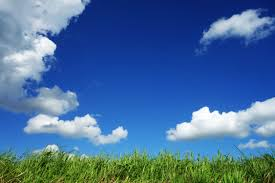
\includegraphics[width=150pt,height=150pt]{images/sunnysky}};


            \draw[fill=black!30, rounded corners] (0.8, 8.2) rectangle (5.2, 7.8) {};
            \foreach \x in {1,...,5}
            {

            	\draw [->,line width=0.1mm] (\x,8) -- (0,6);
            	\draw [->,line width=0.1mm] (\x,8) -- (1,6);
            	\draw [->,line width=0.1mm] (\x,8) -- (2,6);
            	\draw [->,line width=0.1mm] (\x,8) -- (3,6);
            	\draw [->,line width=0.1mm] (\x,8) -- (4,6);
            	\draw [->,line width=0.1mm] (\x,8) -- (5,6);
            	\draw [->,line width=0.1mm] (\x,8) -- (6,6);
            	\draw [->,line width=0.1mm] (\x,8) -- (0,5);
            	\draw [->,line width=0.1mm] (\x,8) -- (1,5);
            	\draw [->,line width=0.1mm] (\x,8) -- (2,5);
            	\draw [->,line width=0.1mm] (\x,8) -- (3,5);
            	\draw [->,line width=0.1mm] (\x,8) -- (4,5);
            	\draw [->,line width=0.1mm] (\x,8) -- (5,5);
            	\draw [->,line width=0.1mm] (\x,8) -- (6,5);
                \foreach \x in {1,...,5}
            	\foreach \y in {8}
            {
            	\node[hid] (1) at (\x,\y){};
            }
            }
            \foreach \x in {0,...,6}
            \foreach \y in {0,...,6}
            {
                \node[mystyle] (\x-\y) at (\x,\y){};

            }
            
	        \end{tikzpicture}
	        \end{center}
		\end{overlayarea}
		\column{0.6\textwidth}
		\begin{overlayarea}{\textwidth}{\textheight}
			\begin{itemize}\justifying
				\item<1-> First let us talk about \textit{abstraction}
				\item<2->  Suppose, we are able to learn the joint distribution $P(V,H)$
				\item<3-> Using this distribution we can find 
				\begin{align*}
				P(H|V) = \frac{P(V,H)}{\sum_H P(V,H)}
				\end{align*}
				\item<4-> In other words, given an image, we can find the most likely latent configuration $(H=h)$ that generated this image (of course, keeping the computational cost aside for now)
				\item<5-> What does this $h$ capture? \onslide<6->{It captures a latent representation or abstraction of the image!}
			\end{itemize}
		\end{overlayarea}
	\end{columns}
\end{frame}


\begin{frame}
	\begin{columns}
		\column{0.4\textwidth}
		\begin{overlayarea}{\textwidth}{\textheight}
		\begin{figure}
		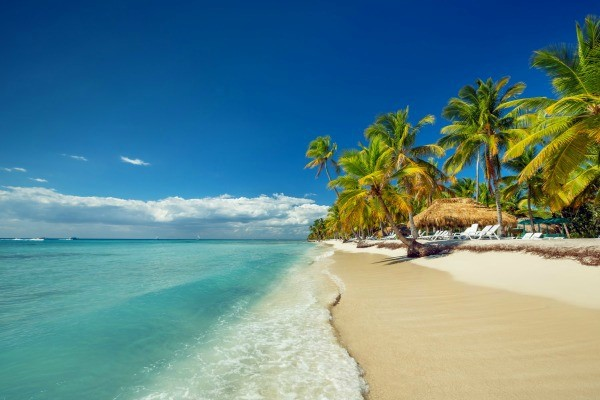
\includegraphics[height=100pt,width=100pt]{images/cloudybeach1}
		\end{figure}
		\end{overlayarea}
		\column{0.6\textwidth}
		\begin{overlayarea}{\textwidth}{\textheight}
			\begin{itemize}\justifying
				\item<1-> In other words, it captures the most important properties of the image
				\item<2-> For example, if you were to describe the adjacent image you wouldn't say ``I am  looking at an image where pixel 1 is blue, pixel 2 is blue, ..., pixel 1024 is beige"
				\item<3->Instead you would just say ``I am looking at an image of a \color{red}{sunny beach} \color{black}{with an} \color{red}{ocean} \color{black}{in the background and} \color{red}{beige sand}\color{black}''
				\item<4->This is exactly the abstraction captured by the vector $h$
			\end{itemize}
		\end{overlayarea}
	\end{columns}
\end{frame}

\begin{frame}
	\begin{columns}
		\column{0.4\textwidth}
		\begin{overlayarea}{\textwidth}{\textheight}
		\begin{figure}
		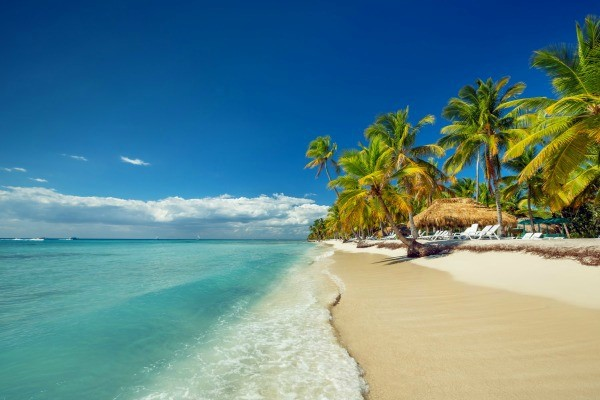
\includegraphics[height=100pt,width=100pt]{images/cloudybeach1}
		\end{figure}

		\begin{minipage}{1\linewidth}
		\begin{minipage}{0.45\linewidth}
		\begin{figure}
		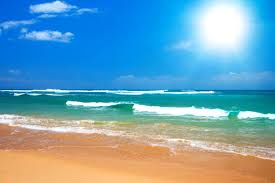
\includegraphics[height=50pt,width=50pt]{images/cloudybeach}
		\end{figure}
		\end{minipage}
		\begin{minipage}{0.45\linewidth}
		\begin{figure}
		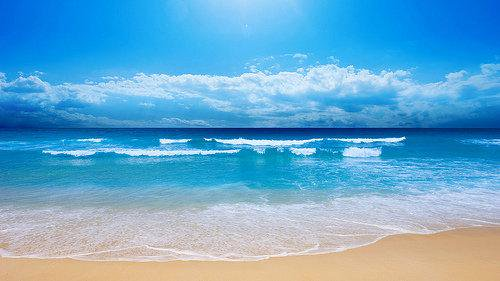
\includegraphics[height=50pt,width=50pt]{images/cloudybeach2}
		\end{figure}
		\end{minipage}
		\end{minipage}	
		\vspace{-0.05in}

		\begin{minipage}{1\linewidth}
		\begin{minipage}{0.45\linewidth}
		\begin{figure}
		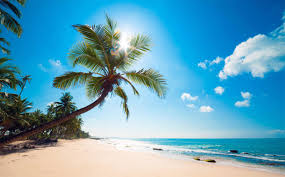
\includegraphics[height=50pt,width=50pt]{images/cloudybeach3}
		\end{figure}
		\end{minipage}
		\begin{minipage}{0.45\linewidth}
		\begin{figure}
		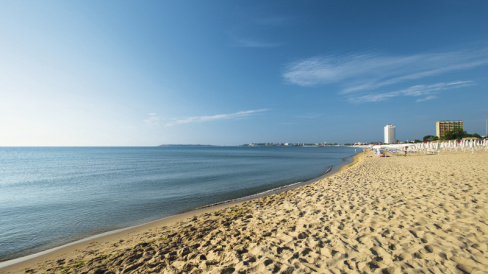
\includegraphics[height=50pt,width=50pt]{images/cloudybeach4}
		\end{figure}
		\end{minipage}
		\end{minipage}
		\end{overlayarea}
		\column{0.6\textwidth}
		\begin{overlayarea}{\textwidth}{\textheight}
			\begin{itemize}\justifying
				\item<1-> Under this abstraction all these images would look very similar (i.e., they would have very similar latent configurations $h$)
				\item<2-> Even though in the original feature space (pixels) there is a significant difference between these images, in the latent space they would be very close to each other
				\item<3-> This is very similar to the idea behind PCA and autoencoders
			\end{itemize}
		\end{overlayarea}
	\end{columns}
\end{frame}


\begin{frame}
	\begin{columns}
		\column{0.4\textwidth}
		\begin{overlayarea}{\textwidth}{\textheight}
			\vspace{0.1in}
			\tikzset{mystyle/.style={shape=circle,fill=black,scale=0.3}}
			\tikzset{neigh/.style={shape=circle,fill=blue,scale=0.5}}
			\tikzset{cent/.style={shape=circle,fill=red,scale=0.5}}
			\tikzset{hid/.style={shape=circle,fill=green,scale=0.5}}
			\tikzstyle{input_neuron}=[circle,draw=red!50,fill=orange!10,thick,minimum size=3mm]
			\begin{center}
			\begin{tikzpicture}[scale=.7]
            % setup the nodes
          	\node[inner sep=0,opacity=0.3] at (3,3)
			{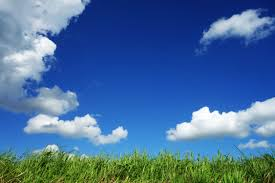
\includegraphics[width=150pt,height=150pt]{images/sunnysky}};


            \draw[fill=black!30, rounded corners] (0.8, 8.2) rectangle (5.2, 7.8) {};
            \foreach \x in {1,...,5}
            {

            	\draw [->,line width=0.1mm] (\x,8) -- (0,6);
            	\draw [->,line width=0.1mm] (\x,8) -- (1,6);
            	\draw [->,line width=0.1mm] (\x,8) -- (2,6);
            	\draw [->,line width=0.1mm] (\x,8) -- (3,6);
            	\draw [->,line width=0.1mm] (\x,8) -- (4,6);
            	\draw [->,line width=0.1mm] (\x,8) -- (5,6);
            	\draw [->,line width=0.1mm] (\x,8) -- (6,6);
            	\draw [->,line width=0.1mm] (\x,8) -- (0,5);
            	\draw [->,line width=0.1mm] (\x,8) -- (1,5);
            	\draw [->,line width=0.1mm] (\x,8) -- (2,5);
            	\draw [->,line width=0.1mm] (\x,8) -- (3,5);
            	\draw [->,line width=0.1mm] (\x,8) -- (4,5);
            	\draw [->,line width=0.1mm] (\x,8) -- (5,5);
            	\draw [->,line width=0.1mm] (\x,8) -- (6,5);
                \foreach \x in {1,...,5}
            	\foreach \y in {8}
            {
            	\node[hid] (1) at (\x,\y){};
            }
            }
            \foreach \x in {0,...,6}
            \foreach \y in {0,...,6}
            {
                \node[mystyle] (\x-\y) at (\x,\y){};

            }
            
	        \end{tikzpicture}
	        \end{center}
		\end{overlayarea}
		\column{0.6\textwidth}
		\begin{overlayarea}{\textwidth}{\textheight}
			\begin{itemize}\justifying
				\item<1-> Of course, we still need to figure out a way of computing $P(H|V)$
				\item<2-> In the case of PCA, learning such latent representations boiled down to learning the eigen vectors of $X^\top X$ (using linear algebra)
				\item<3-> In the case of Autoencoders, this boiled down to learning the parameters of the feedforward network $(W_{end}, W_{dec})$ (using gradient descent)
				\item<4-> We still haven't seen how to learn the parameters of $P(H, V)$ (we are far from it but we will get there soon!)
			\end{itemize}
		\end{overlayarea}
	\end{columns}
\end{frame}

\begin{frame}
	\begin{columns}
		\column{0.4\textwidth}
		\begin{overlayarea}{\textwidth}{\textheight}
			\vspace{0.1in}
			\tikzset{mystyle/.style={shape=circle,fill=black,scale=0.3}}
			\tikzset{neigh/.style={shape=circle,fill=blue,scale=0.5}}
			\tikzset{cent/.style={shape=circle,fill=red,scale=0.5}}
			\tikzset{hid/.style={shape=circle,fill=green,scale=0.5}}
			\tikzstyle{input_neuron}=[circle,draw=red!50,fill=orange!10,thick,minimum size=3mm]
			\begin{center}
			\begin{tikzpicture}[scale=.7]
            % setup the nodes
          	\node[inner sep=0,opacity=0.3] at (3,3)
			{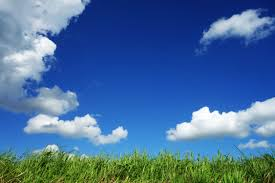
\includegraphics[width=150pt,height=150pt]{images/sunnysky}};


            \draw[fill=black!30, rounded corners] (0.8, 8.2) rectangle (5.2, 7.8) {};
            \foreach \x in {1,...,5}
            {

            	\draw [->,line width=0.1mm] (\x,8) -- (0,6);
            	\draw [->,line width=0.1mm] (\x,8) -- (1,6);
            	\draw [->,line width=0.1mm] (\x,8) -- (2,6);
            	\draw [->,line width=0.1mm] (\x,8) -- (3,6);
            	\draw [->,line width=0.1mm] (\x,8) -- (4,6);
            	\draw [->,line width=0.1mm] (\x,8) -- (5,6);
            	\draw [->,line width=0.1mm] (\x,8) -- (6,6);
            	\draw [->,line width=0.1mm] (\x,8) -- (0,5);
            	\draw [->,line width=0.1mm] (\x,8) -- (1,5);
            	\draw [->,line width=0.1mm] (\x,8) -- (2,5);
            	\draw [->,line width=0.1mm] (\x,8) -- (3,5);
            	\draw [->,line width=0.1mm] (\x,8) -- (4,5);
            	\draw [->,line width=0.1mm] (\x,8) -- (5,5);
            	\draw [->,line width=0.1mm] (\x,8) -- (6,5);
                \foreach \x in {1,...,5}
            	\foreach \y in {8}
            {
            	\node[hid] (1) at (\x,\y){};
            }
            }
            \foreach \x in {0,...,6}
            \foreach \y in {0,...,6}
            {
                \node[mystyle] (\x-\y) at (\x,\y){};

            }
            
	        \end{tikzpicture}
	        \end{center}
		\end{overlayarea}
		\column{0.6\textwidth}
		\begin{overlayarea}{\textwidth}{\textheight}
			\begin{itemize}\justifying
				\footnotesize
				\item<1-> Ok, I am just going to drag this a bit more! (bear with me)
				\item<2-> Remember that in practice we have no clue what these hidden variables are!
				\item<3-> Even in PCA, once we are given the new dimensions we have no clue what these dimensions actually mean 
				\item<4-> We cannot interpret them (for example, we cannot say dimension 1 corresponds to weight, dimension 2 corresponds to height and so on!)
				\item<5->  Even here, we just assume there are some latent variables which capture the essence of the data but we do not really know what these are (because no one ever tells us what these are)
				\item<6-> Only for illustration purpose we assumed that $h_1$ corresponds to sunny/cloudy, $h_2$ corresponds to beach and so on
			\end{itemize}
		\end{overlayarea}
	\end{columns}
\end{frame}

\begin{frame}
	\begin{columns}
		\column{0.4\textwidth}
		\vspace{0.1in}
		\begin{overlayarea}{\textwidth}{\textheight}
			\tikzset{mystyle/.style={shape=circle,fill=black,scale=0.3}}
			\tikzset{neigh/.style={shape=circle,fill=blue,scale=0.5}}
			\tikzset{cent/.style={shape=circle,fill=red,scale=0.5}}
			\tikzset{hid/.style={shape=circle,fill=green,scale=0.5}}
			\tikzstyle{input_neuron}=[circle,draw=red!50,fill=orange!10,thick,minimum size=3mm]
			\begin{center}
			\begin{tikzpicture}[scale=.7]
            % setup the nodes
          	\node[inner sep=0,opacity=0.3] at (3,3)
			{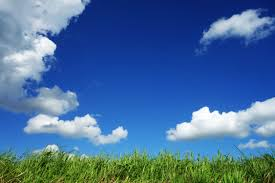
\includegraphics[width=150pt,height=150pt]{images/sunnysky}};


            \draw[fill=black!30, rounded corners] (0.8, 8.2) rectangle (5.2, 7.8) {};
            \foreach \x in {1,...,5}
            {

            	\draw [->,line width=0.1mm] (\x,8) -- (0,6);
            	\draw [->,line width=0.1mm] (\x,8) -- (1,6);
            	\draw [->,line width=0.1mm] (\x,8) -- (2,6);
            	\draw [->,line width=0.1mm] (\x,8) -- (3,6);
            	\draw [->,line width=0.1mm] (\x,8) -- (4,6);
            	\draw [->,line width=0.1mm] (\x,8) -- (5,6);
            	\draw [->,line width=0.1mm] (\x,8) -- (6,6);
            	\draw [->,line width=0.1mm] (\x,8) -- (0,5);
            	\draw [->,line width=0.1mm] (\x,8) -- (1,5);
            	\draw [->,line width=0.1mm] (\x,8) -- (2,5);
            	\draw [->,line width=0.1mm] (\x,8) -- (3,5);
            	\draw [->,line width=0.1mm] (\x,8) -- (4,5);
            	\draw [->,line width=0.1mm] (\x,8) -- (5,5);
            	\draw [->,line width=0.1mm] (\x,8) -- (6,5);
                \foreach \x in {1,...,5}
            	\foreach \y in {8}
            {
            	\node[hid] (1) at (\x,\y){};
            }
            }
            \foreach \x in {0,...,6}
            \foreach \y in {0,...,6}
            {
                \node[mystyle] (\x-\y) at (\x,\y){};

            }
            
	        \end{tikzpicture}
	        \end{center}
		\end{overlayarea}
		\column{0.6\textwidth}
		\begin{overlayarea}{\textwidth}{\textheight}
			\begin{itemize}\justifying
				\item<1-> Just to reiterate, remember that while sending us the wallpaper images our friend never told us what latent variables he/she considered
				\item<2-> Maybe our friend had the following latent variables in mind: $h_1 = cheerful$, $h_2 = romantic$, and so on
				\item<3-> In fact, it doesn't really matter what the interpretation of these latent variable is 
				\item<4-> All we care about is that they should help us learn a good abstraction of the data
				\item<5-> How? \onslide<+->{(we will get there eventually)}
			\end{itemize}
		\end{overlayarea}
	\end{columns}
\end{frame}


\begin{frame}
	\begin{columns}
		\column{0.4\textwidth}
		\begin{overlayarea}{\textwidth}{\textheight}
			\vspace{0.1in}
			\tikzset{mystyle/.style={shape=circle,fill=black,scale=0.3}}
			\tikzset{neigh/.style={shape=circle,fill=blue,scale=0.5}}
			\tikzset{cent/.style={shape=circle,fill=red,scale=0.5}}
			\tikzset{hid/.style={shape=circle,fill=green,scale=0.5}}
			\tikzstyle{input_neuron}=[circle,draw=red!50,fill=orange!10,thick,minimum size=3mm]
			\begin{center}
			\begin{tikzpicture}[scale=.7]
            % setup the nodes
          	\node[inner sep=0,opacity=0.3] at (3,3)
			{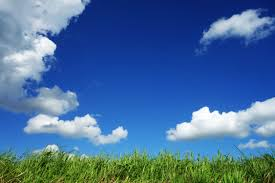
\includegraphics[width=150pt,height=150pt]{images/sunnysky}};


            \draw[fill=black!30, rounded corners] (0.8, 8.2) rectangle (5.2, 7.8) {};
            \foreach \x in {1,...,5}
            {

            	\draw [->,line width=0.1mm] (\x,8) -- (0,6);
            	\draw [->,line width=0.1mm] (\x,8) -- (1,6);
            	\draw [->,line width=0.1mm] (\x,8) -- (2,6);
            	\draw [->,line width=0.1mm] (\x,8) -- (3,6);
            	\draw [->,line width=0.1mm] (\x,8) -- (4,6);
            	\draw [->,line width=0.1mm] (\x,8) -- (5,6);
            	\draw [->,line width=0.1mm] (\x,8) -- (6,6);
            	\draw [->,line width=0.1mm] (\x,8) -- (0,5);
            	\draw [->,line width=0.1mm] (\x,8) -- (1,5);
            	\draw [->,line width=0.1mm] (\x,8) -- (2,5);
            	\draw [->,line width=0.1mm] (\x,8) -- (3,5);
            	\draw [->,line width=0.1mm] (\x,8) -- (4,5);
            	\draw [->,line width=0.1mm] (\x,8) -- (5,5);
            	\draw [->,line width=0.1mm] (\x,8) -- (6,5);
                \foreach \x in {1,...,5}
            	\foreach \y in {8}
            {
            	\node[hid] (1) at (\x,\y){};
            }
            }
            \foreach \x in {0,...,6}
            \foreach \y in {0,...,6}
            {
                \node[mystyle] (\x-\y) at (\x,\y){};

            }
            
	        \end{tikzpicture}
	        \end{center}
		\end{overlayarea}
		\column{0.6\textwidth}
		\begin{overlayarea}{\textwidth}{\textheight}
			\begin{itemize}\justifying
				\item<1-> We will now talk about another interesting concept related to latent variables: \textit{generation}
				\item<2-> Once again, assume that we are able to learn the joint distribution $P(V,H)$
				\item<3-> Using this distribution we can find 
				\begin{align*}
				P(V|H) = \frac{P(V,H)}{\sum_V P(V,H)}
				\end{align*}
				\item<4-> Why is this interesting?
			\end{itemize}
		\end{overlayarea}
	\end{columns}
\end{frame}


\begin{frame}
	\begin{columns}
		\column{0.4\textwidth}
		\begin{overlayarea}{\textwidth}{\textheight}
			\vspace{0.1in}	
			\tikzset{mystyle/.style={shape=circle,fill=black,scale=0.3}}
			\tikzset{neigh/.style={shape=circle,fill=blue,scale=0.5}}
			\tikzset{cent/.style={shape=circle,fill=red,scale=0.5}}
			\tikzset{hid/.style={shape=circle,fill=green,scale=0.5}}
			\tikzstyle{input_neuron}=[circle,draw=red!50,fill=orange!10,thick,minimum size=3mm]
			\begin{center}
			\begin{tikzpicture}[scale=.7]
            % setup the nodes
          	\node[inner sep=0,opacity=0.3] at (3,3)
			{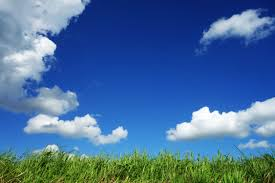
\includegraphics[width=150pt,height=150pt]{images/sunnysky}};


            \draw[fill=black!30, rounded corners] (0.8, 8.2) rectangle (5.2, 7.8) {};
            \foreach \x in {1,...,5}
            {

            	\draw [->,line width=0.1mm] (\x,8) -- (0,6);
            	\draw [->,line width=0.1mm] (\x,8) -- (1,6);
            	\draw [->,line width=0.1mm] (\x,8) -- (2,6);
            	\draw [->,line width=0.1mm] (\x,8) -- (3,6);
            	\draw [->,line width=0.1mm] (\x,8) -- (4,6);
            	\draw [->,line width=0.1mm] (\x,8) -- (5,6);
            	\draw [->,line width=0.1mm] (\x,8) -- (6,6);
            	\draw [->,line width=0.1mm] (\x,8) -- (0,5);
            	\draw [->,line width=0.1mm] (\x,8) -- (1,5);
            	\draw [->,line width=0.1mm] (\x,8) -- (2,5);
            	\draw [->,line width=0.1mm] (\x,8) -- (3,5);
            	\draw [->,line width=0.1mm] (\x,8) -- (4,5);
            	\draw [->,line width=0.1mm] (\x,8) -- (5,5);
            	\draw [->,line width=0.1mm] (\x,8) -- (6,5);
                \foreach \x in {1,...,5}
            	\foreach \y in {8}
            {
            	\node[hid] (1) at (\x,\y){};
            }
            }
            \foreach \x in {0,...,6}
            \foreach \y in {0,...,6}
            {
                \node[mystyle] (\x-\y) at (\x,\y){};

            }
            
	        \end{tikzpicture}
	        \end{center}
		\end{overlayarea}
		\column{0.6\textwidth}
		\begin{overlayarea}{\textwidth}{\textheight}
			\begin{itemize}\justifying
				\item<1->  Well, I can now say ``Create an image which is cloudy, has a beach and depicts daytime''
				\item<2-> Or given $h = [....]$ find the corresponding $V$ which maximizes $P(V|H)$
				\item<3-> In other words, I can now generate images given certain latent variables
				\item<4-> The hope is that I should be able to ask the model to generate very creative images given some latent configuration (we will come back to this later)
			\end{itemize}
		\end{overlayarea}
	\end{columns}
\end{frame}

\begin{frame}
\begin{block}{The story ahead...}
\begin{itemize}	
	 \item<1-> We have tried to understand the intuition behind latent variables and how they could potenatially allow us to do abstraction and generation
	\item<2-> We will now concretize these intuitions by developings equations (models) and learning algoritms 
	\item<3-> And of course, we will tie all this back to neural networks!
	\end{itemize}
\end{block}
\end{frame}

\begin{frame}
	\begin{block}{}
		\begin{itemize}
			\item<1-> For the remainder of this discussion we will assume that all our variables take only boolean values
			\item<2-> Thus, the vector $V$ will be a boolean vector $\in \{0, 1\}^m$ (there are a total of $2^m$ values that $V$ can take)
			\item<3-> And the vector $H$ will be a boolean vector $\in \{0, 1\}^n$ (there are a total of $2^n$ values that $H$ can take)
		\end{itemize}
	\end{block}
\end{frame}
